\documentclass[10pt]{article}
\usepackage[margin=1in]{geometry}
\usepackage{graphicx}
\usepackage{booktabs}
\usepackage{hyperref}
\usepackage{amsmath}

\title{Task-Based Parallel Runtime with a Work-Stealing Scheduler}
\author{Your Name}
\date{\today}

\begin{document}
\maketitle

\begin{abstract}
Task-based execution is a widely used shared-memory parallel programming model because it decouples application structure from low-level thread management. This project presents a compact C++17 task runtime for directed acyclic graph (DAG) workloads that combines dependency-aware scheduling with a decentralized work-stealing policy. The runtime uses a fixed-size thread pool, per-worker double-ended queues, atomic dependency counters, and lightweight condition-variable coordination. We evaluate the implementation on three representative workloads: parallel sum, blocked matrix multiplication, and a synthetic multi-stage DAG. Across 1, 2, 4, and 8 worker threads, the system achieves up to $5.74\times$ speedup on the reduction workload, $4.84\times$ on matrix multiplication, and $5.14\times$ on the synthetic DAG. The results show that even a relatively small runtime can expose meaningful parallel scalability while maintaining a clear software structure suitable for experimentation and teaching.
\end{abstract}

\section{Introduction}
Modern multicore processors offer substantial thread-level parallelism, but programming them efficiently remains challenging. Explicit thread management often entangles algorithm logic with synchronization, load balancing, and execution policy. Task-based runtimes address this problem by allowing the programmer to describe units of work and dependencies between them while the runtime schedules ready tasks onto available worker threads.

This preprint studies a lightweight shared-memory task runtime implemented in modern C++. The goal is not to compete with production-grade systems, but to build a research-oriented prototype that exposes the core mechanisms behind DAG execution and work stealing in a form that is easy to inspect, benchmark, and extend. The project is motivated by three questions: how to represent dependency-constrained tasks cleanly, how to schedule them with minimal centralized control, and how effectively such a design scales on representative workloads.

The main contributions of the project are:
\begin{itemize}
    \item a modular C++17 runtime that executes task graphs with explicit dependencies;
    \item a work-stealing scheduler based on per-worker deques and a fixed thread pool;
    \item a benchmark suite covering reduction, dense numerical computation, and irregular DAG execution; and
    \item a reproducible analysis pipeline that exports CSV measurements and generates plots for both a paper and a project website.
\end{itemize}

\section{Background}
In a task-based parallel model, computation is decomposed into tasks that may execute when their input dependencies are satisfied. A natural representation is a directed acyclic graph, where vertices correspond to tasks and edges encode precedence constraints. A scheduler must identify ready tasks, dispatch them to workers, and activate successor tasks as dependencies complete.

Work stealing is a common approach for balancing load in such systems. Rather than maintaining a single global queue, each worker owns a local task deque. Workers preferentially execute local work, which preserves locality and reduces contention, while idle workers steal tasks from others. This decentralized structure performs especially well when the number of ready tasks varies over time or when parallelism is unevenly distributed across the DAG.

\section{System Design}
The runtime is organized around four central abstractions.

\textbf{Task graph.} Each task is represented as a node containing a callable function, a list of successor task identifiers, and an atomic counter recording the number of unresolved predecessor dependencies. The graph is constructed before execution begins.

\textbf{Thread pool.} A fixed number of worker threads is created during runtime initialization. Workers persist for the lifetime of the runtime and repeatedly look for ready tasks until all work is complete.

\textbf{Per-worker queues.} Each worker owns a double-ended queue protected by a mutex. Local execution follows a last-in, first-out policy by popping from the back of the worker's own deque. This favors recently spawned tasks and improves temporal locality.

\textbf{Work stealing.} When a worker's local queue is empty, it randomly probes peer workers and steals from the front of a victim deque. This front-steal/back-pop discipline reduces interference with local execution while enabling dynamic balancing.

The execution policy is dependency driven. At startup, tasks with zero unresolved dependencies are inserted into worker queues. When a worker completes a task, the runtime decrements the counters of each successor. Any successor whose counter reaches zero becomes ready and is enqueued for future execution.

\section{Implementation}
The runtime interface is intentionally small. The user creates tasks, adds dependency edges, starts execution, and then blocks until completion. Internally, the implementation relies on standard C++ concurrency primitives:
\begin{itemize}
    \item \texttt{std::thread} for the worker pool,
    \item \texttt{std::atomic} for dependency counters and completion tracking,
    \item \texttt{std::mutex} for queue protection, and
    \item \texttt{std::condition\_variable} for coordinating worker sleep and wake-up.
\end{itemize}

Task storage is separated from ready-queue management. This avoids coupling graph structure to instantaneous scheduling state and keeps queue operations small. The implementation also uses a deque-based task container so task identifiers remain stable after insertion, which simplifies dependency bookkeeping.

The scheduler loop follows a simple sequence:
\begin{enumerate}
    \item attempt to pop a task from the local worker deque;
    \item if no local work is available, attempt to steal from another worker;
    \item if a task is found, execute it and update successor dependency counters;
    \item if no work is available anywhere, wait on a condition variable until new tasks become ready or execution finishes.
\end{enumerate}

This design intentionally prioritizes clarity over advanced optimizations such as lock-free queues, NUMA awareness, or adaptive stealing heuristics. That tradeoff is appropriate for a research prototype whose purpose is to make scheduler behavior visible and measurable.

\section{Experimental Methodology}
The benchmark suite evaluates the runtime using 1, 2, 4, and 8 worker threads. Each configuration is executed three times, and the median runtime is reported to reduce the impact of transient noise.

Three workloads are used:
\begin{itemize}
    \item \textbf{Parallel sum:} a large array is partitioned into chunks, each chunk is reduced independently, and a tree of reduction tasks produces the final sum.
    \item \textbf{Matrix multiplication:} a dense matrix product is decomposed into row-block tasks, yielding mostly independent parallel work with regular computational structure.
    \item \textbf{Synthetic DAG:} a staged task graph with cross-stage dependencies is used to stress the scheduler under less regular ready-task patterns.
\end{itemize}

For each workload and thread count, the benchmark records execution time in milliseconds. Speedup is defined as
\[
S_p = \frac{T_1}{T_p},
\]
where $T_1$ is the single-thread runtime and $T_p$ is the runtime with $p$ worker threads. Efficiency is defined as
\[
E_p = \frac{S_p}{p}.
\]

\section{Results}
Table~\ref{tab:results} summarizes the measured execution time, speedup, and efficiency. Figure~\ref{fig:time}, Figure~\ref{fig:speedup}, and Figure~\ref{fig:efficiency} visualize the same data.

\begin{table}[h]
    \centering
    \small
    \begin{tabular}{llrrr}
        \toprule
        Workload & Threads & Time (ms) & Speedup & Efficiency \\
        \midrule
        Parallel Sum & 1 & 13.4350 & 1.0000 & 1.0000 \\
        Parallel Sum & 2 & 6.0663 & 2.2147 & 1.1074 \\
        Parallel Sum & 4 & 3.0585 & 4.3926 & 1.0982 \\
        Parallel Sum & 8 & 2.3401 & 5.7412 & 0.7176 \\
        \midrule
        Matrix Multiplication & 1 & 39.9890 & 1.0000 & 1.0000 \\
        Matrix Multiplication & 2 & 20.4895 & 1.9517 & 0.9758 \\
        Matrix Multiplication & 4 & 11.0449 & 3.6206 & 0.9051 \\
        Matrix Multiplication & 8 & 8.2698 & 4.8355 & 0.6044 \\
        \midrule
        Synthetic DAG & 1 & 107.7250 & 1.0000 & 1.0000 \\
        Synthetic DAG & 2 & 55.8647 & 1.9283 & 0.9642 \\
        Synthetic DAG & 4 & 32.0682 & 3.3593 & 0.8398 \\
        Synthetic DAG & 8 & 20.9418 & 5.1440 & 0.6430 \\
        \bottomrule
    \end{tabular}
    \caption{Benchmark results for the task runtime.}
    \label{tab:results}
\end{table}

The parallel sum workload shows the strongest scaling at low and moderate thread counts, reaching $4.39\times$ speedup at 4 threads and $5.74\times$ at 8 threads. This behavior is expected because the workload exposes a large number of independent chunk tasks followed by a structured reduction tree, providing abundant ready work and relatively low synchronization overhead. The efficiency values above 1.0 at 2 and 4 threads should not be interpreted as literal superlinear behavior; instead, they likely reflect measurement noise, cache effects, and the small absolute runtime of the workload.

Matrix multiplication also scales well, although less aggressively than the reduction benchmark. The workload reaches $3.62\times$ speedup at 4 threads and $4.84\times$ at 8 threads. Because each task performs substantial arithmetic on a row block, the scheduler overhead is amortized effectively. However, efficiency declines as thread count increases, suggesting the growing influence of memory-system effects and diminishing marginal parallelism relative to the synchronization and queue-management cost.

The synthetic DAG exhibits the highest absolute runtime in the single-thread case and provides a useful test of irregular scheduling behavior. It achieves $1.93\times$, $3.36\times$, and $5.14\times$ speedup at 2, 4, and 8 threads respectively. Although the scaling is solid, efficiency degrades with thread count, indicating that dependency structure and synchronization increasingly limit parallel utilization when more workers contend for less uniformly available ready work.

Overall, the results show that the runtime captures the expected qualitative behavior of a work-stealing task system. It scales best when the task graph exposes many independent tasks and when task granularity is large enough to amortize scheduling overhead. As concurrency increases, the usual shared-memory bottlenecks become visible: contention, synchronization, and memory traffic reduce efficiency even though total execution time continues to improve.

\begin{figure}[h]
    \centering
    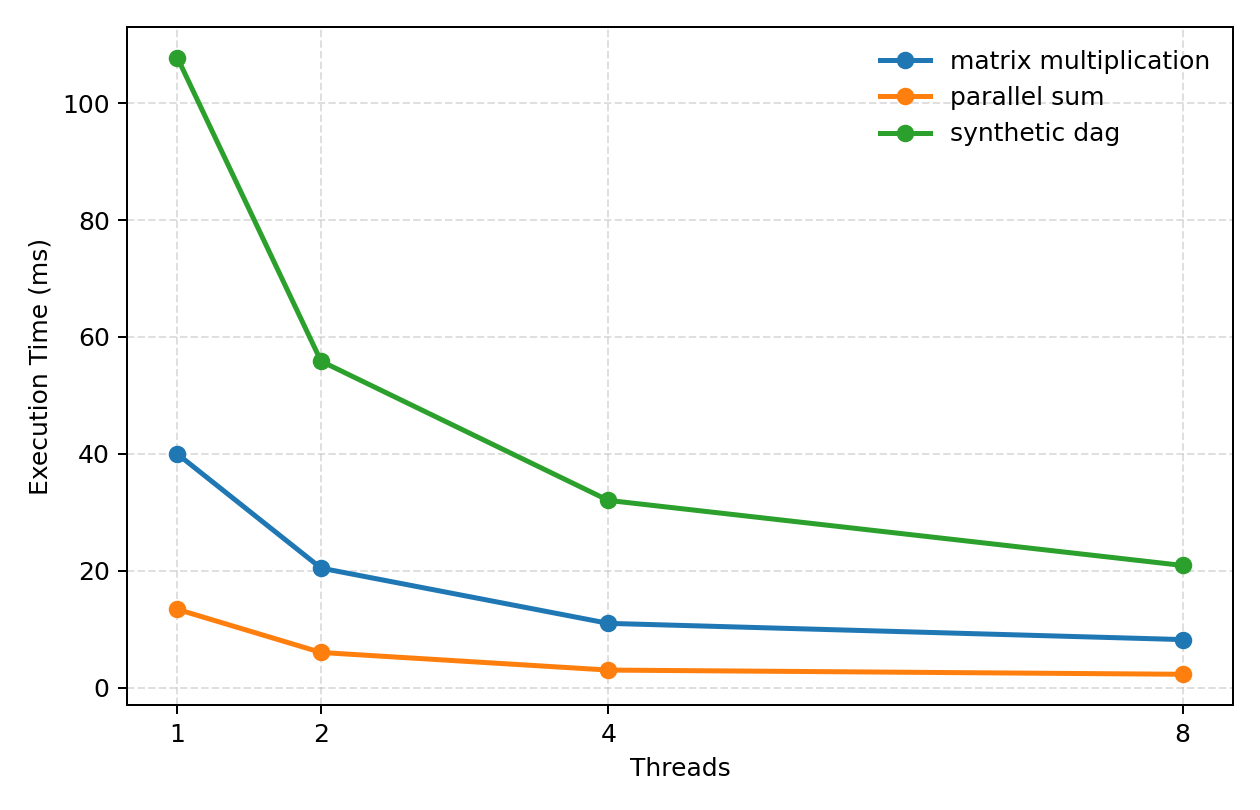
\includegraphics[width=0.8\linewidth]{../results/figures/execution_time.png}
    \caption{Execution time across workloads and thread counts.}
    \label{fig:time}
\end{figure}

\begin{figure}[h]
    \centering
    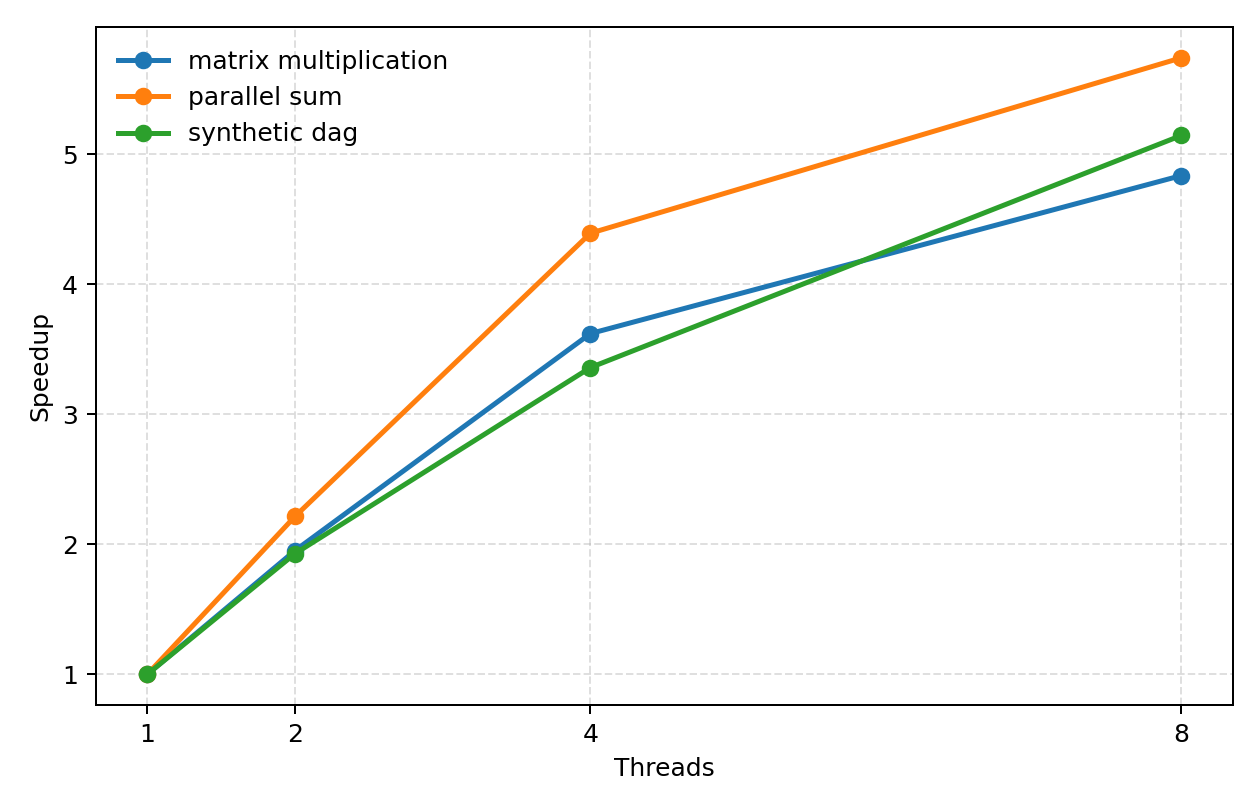
\includegraphics[width=0.8\linewidth]{../results/figures/speedup.png}
    \caption{Speedup across workloads and thread counts.}
    \label{fig:speedup}
\end{figure}

\begin{figure}[h]
    \centering
    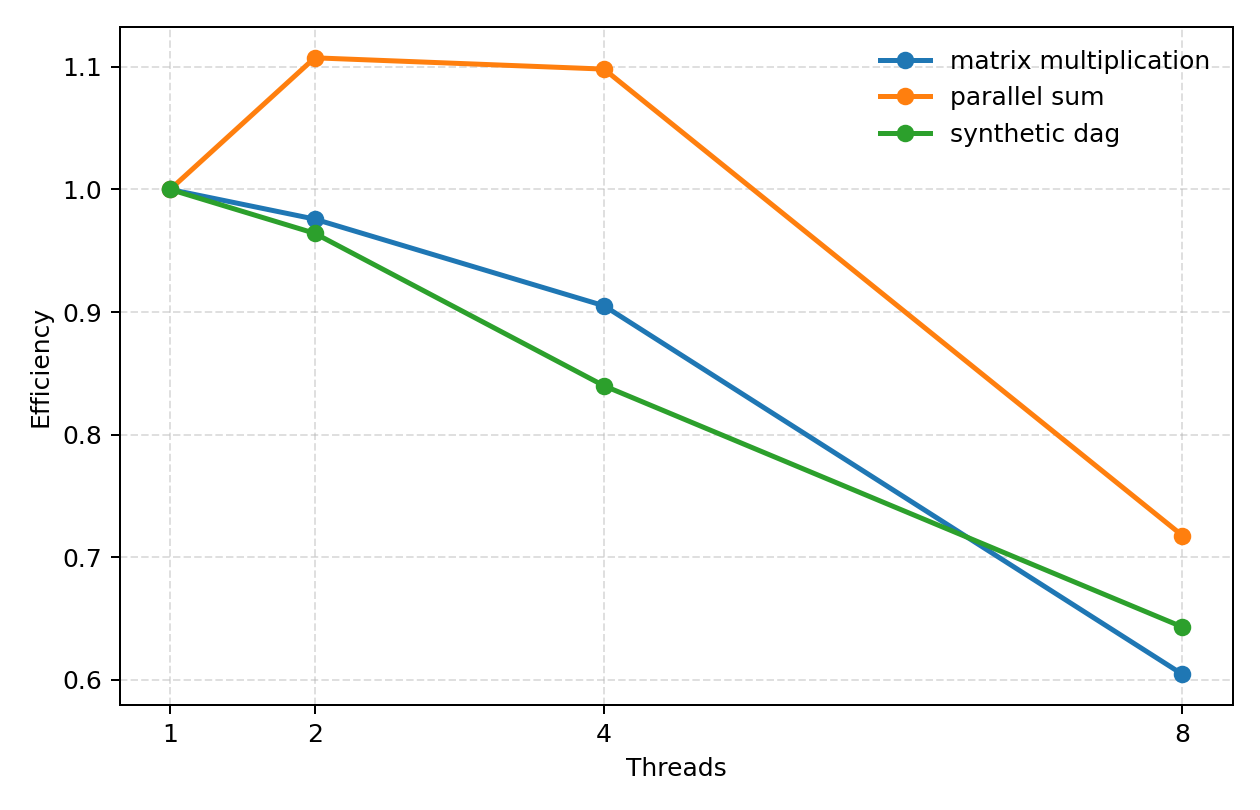
\includegraphics[width=0.8\linewidth]{../results/figures/efficiency.png}
    \caption{Parallel efficiency across workloads and thread counts.}
    \label{fig:efficiency}
\end{figure}

\section{Discussion}
The project demonstrates that a compact implementation can still capture the central ideas of DAG scheduling and work stealing. That makes the codebase useful not only as a functional runtime, but also as a teaching and experimentation platform. At the same time, the current evaluation has clear limitations. The experiments report only a small number of median timings, they do not include variance bars, and they do not compare against a baseline scheduler such as a centralized queue or a purely static partitioning strategy.

These limitations point directly to future work. A stronger study would add repeated trials with confidence intervals, benchmark larger problem sizes, evaluate overhead as a function of task granularity, and compare the work-stealing design to one or more alternative schedulers. It would also be valuable to instrument queue activity and steal counts to relate observed performance directly to scheduler behavior.

\section{Conclusion}
This preprint presented a task-based parallel runtime for shared-memory systems, implemented in C++17 with explicit DAG dependencies and a work-stealing scheduler. The runtime successfully executes three representative workloads and demonstrates meaningful multicore speedup across 1 to 8 worker threads. While intentionally simple, the design captures the core mechanisms of dependency-aware parallel execution and provides a solid foundation for deeper scheduler research, richer benchmarking, and public project presentation through both a paper and a website.

\end{document}
